\section*{Quality Control of raw reads}

We used LongQC and FASTQC to calculate basic technical statistics and evaluate the quality of \ac{HiFi} raw reads~\cite{fukasawaLongQCQualityControl2020,BabrahamBioinformaticsFastQC}. The length of the 1,747,253 raw reads follows a unimodal distribution with a median size of 13.85kb ($\min = 0.10$kb, $\max = 46.7$kb) \\

The quality reports show no issues except for the GC distribution, which exhibited a bimodal distribution with two peaks, around 45 \% and 37 \%, respectively. We trimmed 25 sequences at 3' and 5' using LongQC. Despite the minimal impact of these, we used the trimmed sequences for the remainder of the analysis. \\
%Among  Angiosperm plants, GC content, might show an irregular or bimodal distribution, although most dicots, such as \textit{T. vulgaris}, exhibit more normal distributions.\cite{bowersGCContentPlant2022}

\section*{Exploratory analysis of long reads and reference genome}

When aligning the best five percent of \ac{HiFi} reads to the \textit{T. quinquecostatus} reference genome, we mapped 97.6\% of the reads. The alignment blocks have a median length of 3.2kb ($\min = 0.2$kb, $\max = 61.8$kb). The median theoretical coverage of chromosomes is 18.1x ($\min = 16.3$x, $\max = 20.5$x). \\

However, the genome coverage is not random. As explained in the corresponding section on methods, we fitted a Zero-Inflated Poisson to the counts' distribution per 1000-length windows using Bayesian inference. The posterior sampling distribution of the parameters is shown in \autoref{fig:bayesian_posterior}. The 95 \% credibility interval, computed for all chromosomes, is 0.74-0.77 for $p$, the probability of not coming from the Poisson process, and 2.02-2.51 for $\lambda$, the rate of mapped reads per window. \\

\graphicspath{{gfx/}}
\begin{sidewaysfigure}
\begin{center}
    \input{gfx/05-posterior_var_edited.pdf_tex}
    \caption{Posterior sampling distribution of mapped reads according to a Zero-inflated Poisson process}    
    \label{fig:bayesian_posterior}    
\end{center}
\footnotesize
The posterior sampling distributions were obtained by modeling the number of mapped reads per 1000-length windows according to the model specified by \eqref{eq:model} using \ac{MCMC}.   
\end{sidewaysfigure}    

Although not included in this report, we experimented with different subset sizes, alignment tools, and window sizes. These experiments produced consistent results. Regarding the number of iterations and chains, various experiments with both experimental and simulated data justified a conservative choice, as we obtained equivalent results in all cases using fewer computational resources. \\

\section*{De novo assembly of T. vulgaris and homology-based assembly scaffolding}

As discussed in Methods, we obtained a \textit{de novo} assembly from our \ac{HiFi} reads and generated scaffolds using RagTag, according to a whole-genome alignment of the \textit{de novo} contigs against \textit{T. quinquecostatus} assembly.\\

The covered regions of the \textit{T. quinquecostatus} genome are shown in \autoref{fig:coverage_long_reads}. The alignments cover most of the "telomeric" regions for the 13 pseudo-chromosomes but present large uncovered areas, especially near the middle of the pseudo-chromosome. In total, 47.3\% of the \textit{T. quinquecostatus} genome is uncovered. This fact is consistent with the Zero-inflated poisson model discussed above.\\

\begin{figure}[h]
    \begin{center}
        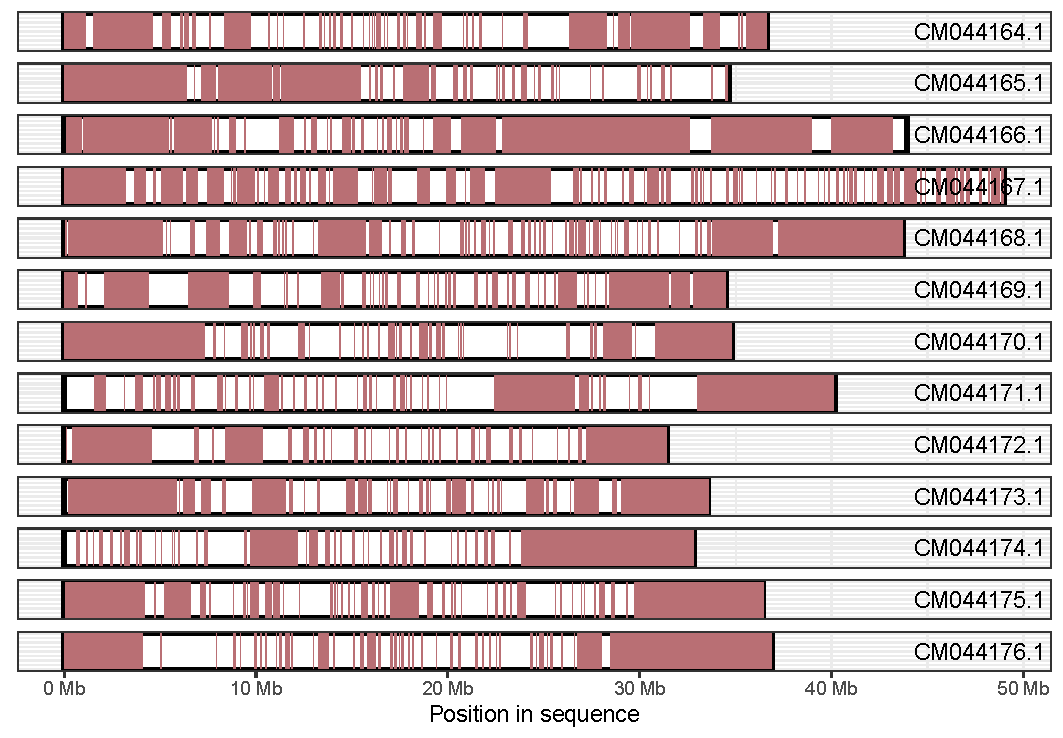
\includegraphics[width=\textwidth]{gfx/coverage_long_reads_tq.pdf}
        \caption{Coverage across \textit{T. quinquecostatus} of the whole-genome alignment between \textit{T. vulgaris} and \textit{T. quinquecostatus}}   
        \label{fig:coverage_long_reads}
 
    \end{center}
        \footnotesize
    We show the covered areas of the \textit{T. quinquecostatus} reference genome in red. We include only the primary alignment whose length is greater than 1000, as those are the ones RagTag will use for the scaffolding process. We represent the alignments only to the 13 pseudo-chromosomes.  
\end{figure}   

We used the whole-genome alignment to orient and arrange the different contigs into bigger scaffolds (see \autoref{fig:sinteny} for an example). We calculated the gap sizes according to Equation \eqref{eq:infergapsize} when possible. In most cases, we could not infer the gap size because the inferred size was greater than the threshold established. In total, 91.7\% of the inferred gaps have an unknown size. By convention, gaps of unknown size have a  length of 100 bp.\cite{AGPSpecificationV2}\\

\begin{figure}
\begin{center}
    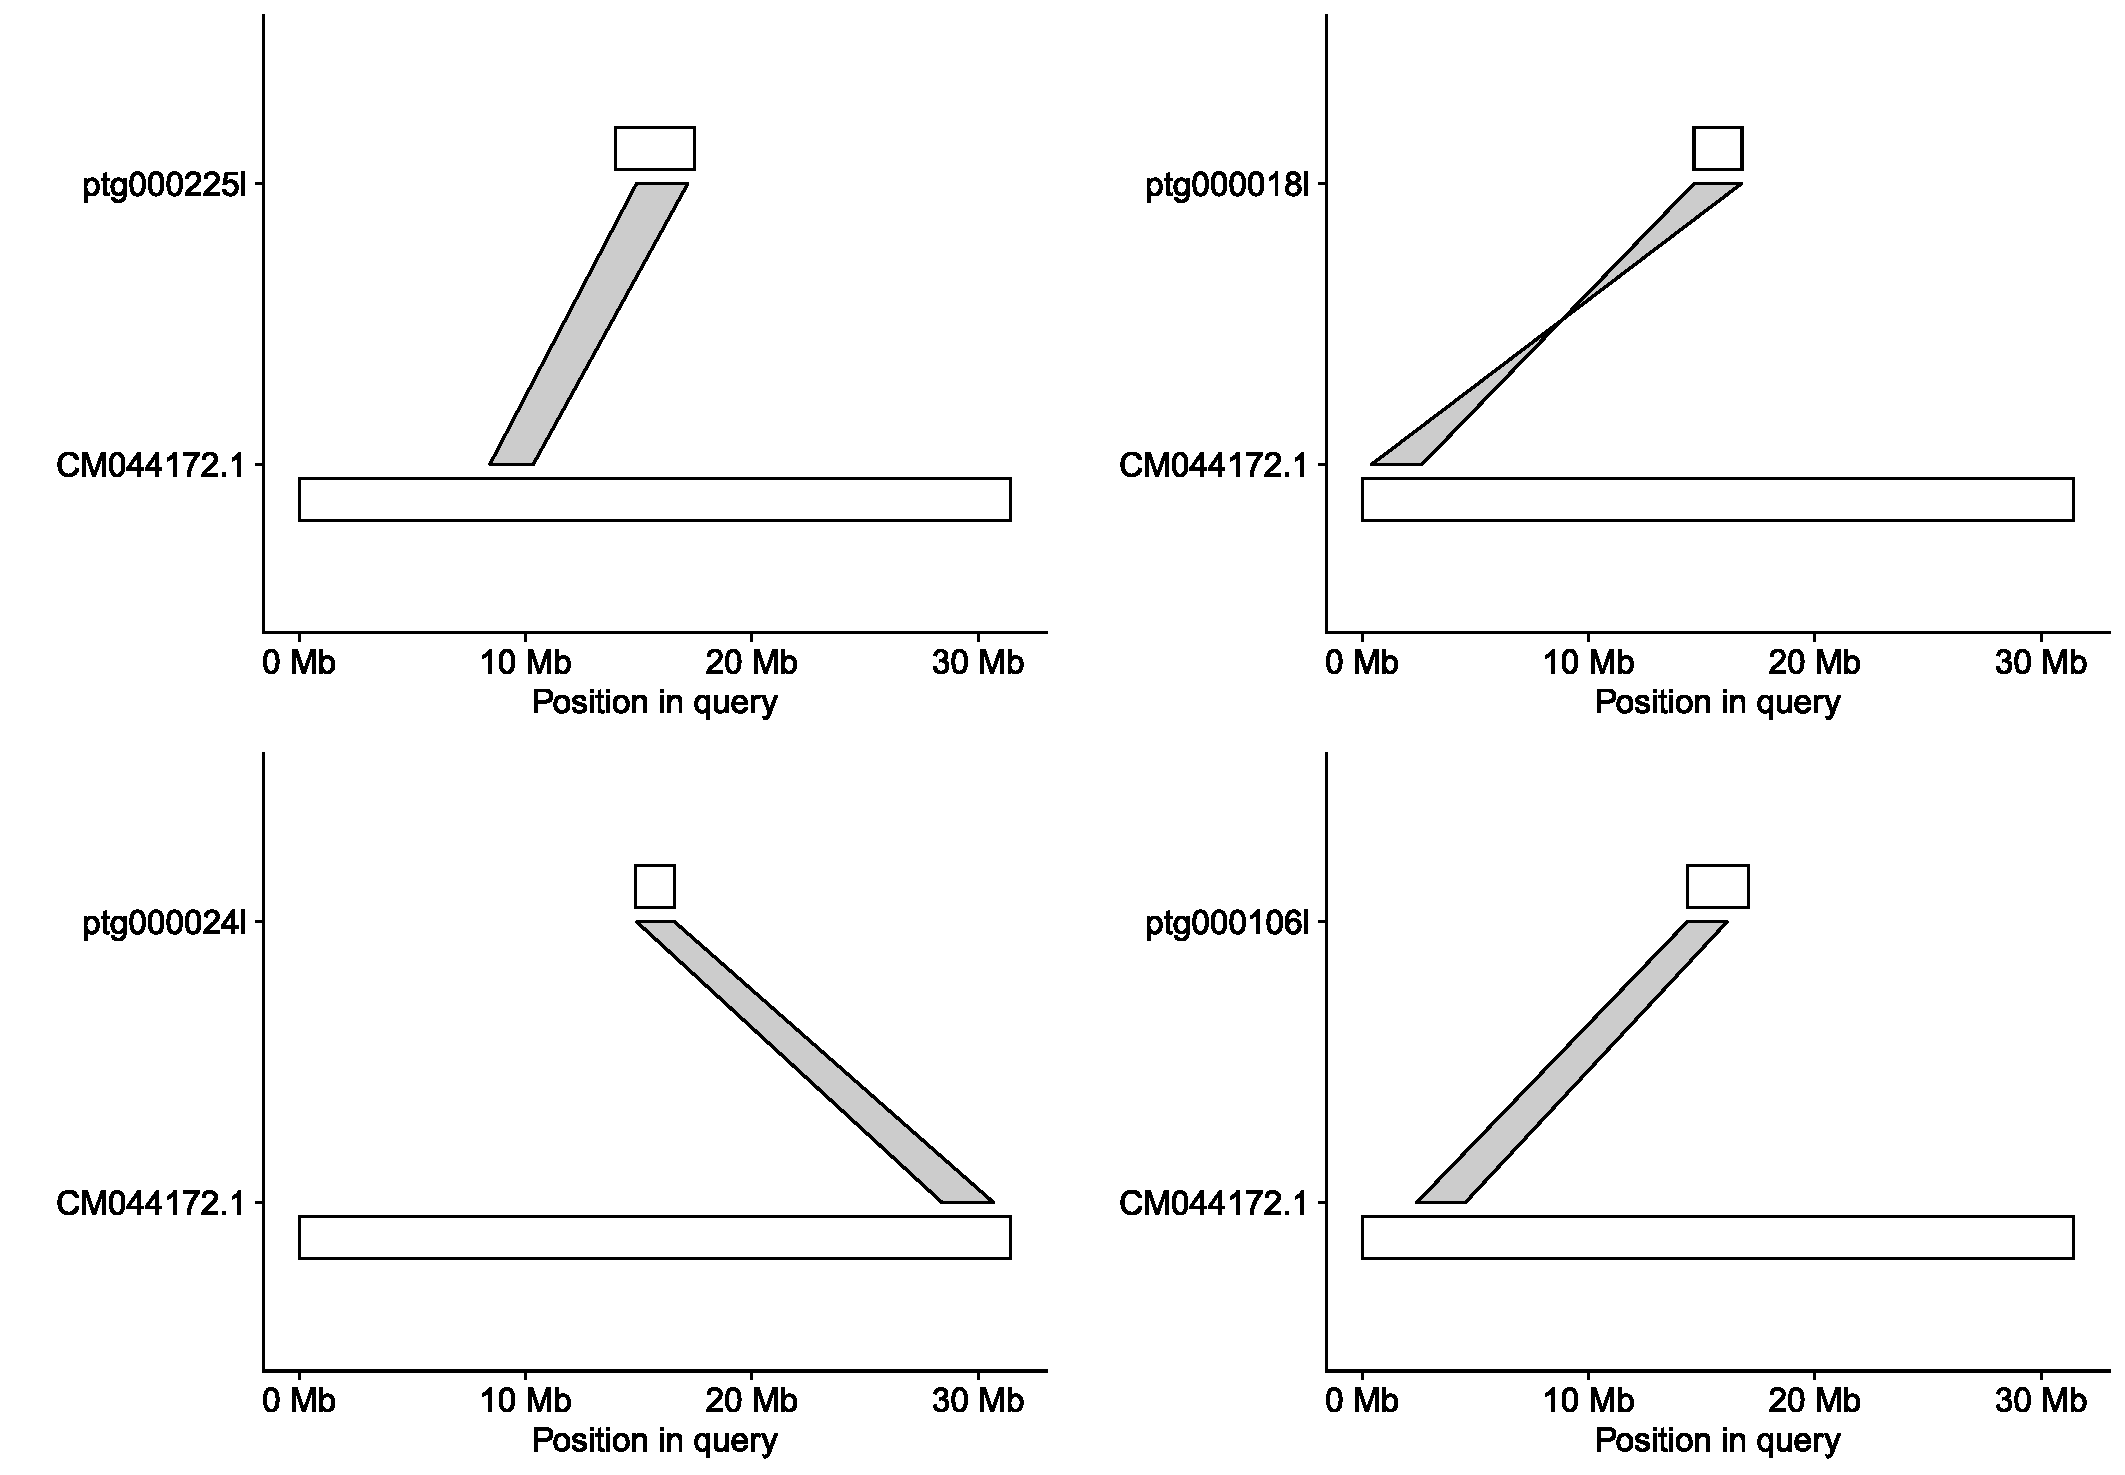
\includegraphics[width=\textwidth]{gfx/CM044172.1_sinteny.pdf}
    \caption{Sinteny-like plot of pseudochromosome CM044172.1}  
    \label{fig:sinteny}    
\end{center}
\footnotesize
We show the alignments of the largest four \textit{de novo} contigs of \textit{T. vulgaris} mapped to \textit{T. quinquecostatus}. This visualization corresponds to arranging and orienting the contigs in the scaffolding process. 
\end{figure} 


The scaffolding process placed 880 contigs (77 \% of base pairs) into bigger scaffolds. Interestingly, a few of the contigs of the draft assembly aligned not to the \textit{T. quinquecostatus} pseudo-chromosomes but to its unplaced contigs.\\

We generated 13 pseudo-chromosomes by joining the adjacent contigs of the draft assembly that aligned to each of the 13 pseudo-chromosomes of \textit{T. quinquecostatus} (supported by \ac{Hi-C} experimental data). This reconstruction is based on the synteny between 
\textit{T. quinquecostatus} and \textit{T. vulgaris}.\\

\section*{Assembly quality assessment}

We show global statistics comparing the assembly at a contig and scaffold level in \autoref{tab:global}. The scaffolding has proven highly effective, as the final assembly has a contig N50 of 1.87 Mb and a scaffold N50 of 48.92 Mb. \\

According to cytometric estimations, the \textit{T. vulgaris} haploid genome size is 754.60 Mb (1C\footnote{The amount of DNA contained within a haploid nucleus} = 0.77pg).~\cite{marieCytometricExercisePlant1993,PlantDNACvalues} The total size of our 13 pseudo-chromosomes is 695.63 Mb. Considering the sum of the 48 scaffolds placed by homology with unplaced \textit{T. quinquecostatus} contigs, the number is closer to the cytometric estimation:  706.41Mb. However, the size of the whole assembly exceeds the estimate; 911.87Mb. This fact supports the reliability of the pseudochromosomes obtained. \\

\begin{table}[h!]
    \begin{minipage}{\linewidth}
    \renewcommand\thefootnote{\thempfootnote}
    \centering
    \begin{tabular}{@{}cccccc@{}}
        \toprule
        & N\#    & Ave (Mb) & Largest (Mb)& N50 (Mb)\footnote{length such that scaffolds/contigs of this length or longer include half the bases of the assembly.}     & Ns\footnote{Number of Ns ambiguous nucleotides}      \\ \midrule
        Contigs      & 1,884 & 0.48     & 11.17        & 1.87 ($n$=133) & 0       \\
        Scaffolds & 1,065 & 0.86     & 95.24        & 48.92 ($n$=8)  & 2,536,928 \\ \bottomrule
        \end{tabular}
        \caption{Global statistics of the assembly at contig and scaffold level}
        \label{tab:global}
\end{minipage}
\end{table}

BUSCO analysis assesses the genome assembly completeness by examining the expected gene content of universal orthologs. The analysis produced the following results: C:96.4\%[S:65.0\%,D:31.4\%], F:0.6\%, M:3.0\%, n:2326.\\

The completeness score, 96.4 \%, is only slightly lower than the one obtained by Sun \etal~\cite{sunChromosomelevelAssemblyAnalysis2022} for \textit{T. quinquecostatus}, which is the closest assembly available. However, the percentage of complete and duplicated genes in \textit{T. vulgaris} is significantly higher at 31.4\% compared to \textit{T. quinquecostatus}, which is only 4.46\%. Using it for scaffolding does not affect this result, as we are not modifying the original sequence.\\


\section*{Mapping short Illumina reads to scaffolded assembly}

\autoref{fig:error_rate} shows the result of mapping the Illumina reads of the five individuals to the scaffolded assembly. Since these reads have been sequenced using baits technology, the coverage cannot be used as a validation of our reference genome. In this case, the low coverage values are because we are not sequencing random samples from the genome but instead capturing particular sequences.\\

%Using hybridization condition one 74.61 \%, of the reference genome is uncovered. Using hybridization condition two, this number is even higher: 92.50\%. Instead, we can observe whether the number of mapped sequences and mismatches conform to expectations.  \\

\begin{figure}
    \begin{center}
        \def\svgwidth{\textwidth}
        \input{gfx/mapped_vs_error_rate.pdf_tex}
        \caption{Results of aligning Illumina short reads to the assembly under two hybridization conditions}            
        \label{fig:error_rate}
    \end{center}
    \footnotesize
    We show the percentage of properly paired reads (with consistent orientation and distance within forward and reverse read) and the percentage of mismatches of the Illumina short reads of 5 different individuals (see \autoref{tab:illumina_samples}). Each specimen was sequenced using two different hybridization protocols for the scaffolded assembly.     
\end{figure}  

The two \textit{S. montana} individuals are grouped in \autoref{fig:error_rate}, showing similar mapping patterns to the scaffolded assembly of \textit{T. vulgaris}. They have a lower percentage of properly mapped sequences than the other \textit{T. vulgaris} specimens. Hybridization two, the more stringent procedure, increases the percentage of mapped reads and the number of mismatches in both \textit{S. montana} individuals.\\

The increased number of mapped reads also affects \textit{T. vulgaris} individuals, but it is less pronounced. Hybridization two does not increase the number of mismatches in \textit{T. vulgaris} as it does in \textit{S. montana}. The differences in the percentage of mapped reads between \textit{T. vulgaris} individuals are slight, but the individual Thym607 used to construct the assembly has the lowest number of mismatches.\\

Although we achieved better mapping results with Thym607 by penalizing SNPs (Single-nucleotide polymorphism) and indels (insertions or deletions) more than the default, we used default parameters for a more appropriate comparison.\\ 